\section{Hasil Simulasi dan Optimasi}
\label{sec:hasil-simulasi-optimasi}

Proses optimasi dilakukan secara simultan dengan simulasi variasi durasi gangguan cuaca dan variasi konsumsi harian BBM. Standar simulasi yang dilakukan dalam pengerjaan tugas akhir ini adalah 1000 iterasi untuk satu kali simulasinya. Skenario yang dilakukan ada dua jenis, yaitu usulan sistem pemasokan baru tanpa pengembangan tangki dan dengan pengembangan tangki penyimpanan di pelabuhannya. Hasil simulasi dapat dilihat pada tabel \ref{tabel:ringkasan-hasil}, sedangkan untuk bentuk distribusi masing-masing variabel dapat dilihat pada pembahasan selanjutnya.

\begin{table}[!ht]
    \centering
    \caption{Ringkasan Hasil Simulasi Skenario}
    \label{tabel:ringkasan-hasil}
    \begin{tabular}{|cccccc|}
    \hline
    \multicolumn{6}{|c|}{TANPA TANGKI}                                                                                                                                                           \\ \hline
    \multicolumn{1}{|c|}{Variabel}                & \multicolumn{1}{c|}{Satuan}      & \multicolumn{1}{c|}{Min.}     & \multicolumn{1}{c|}{Mean}     & \multicolumn{1}{c|}{Max.}     & STD. DEV. \\ \hline
    \multicolumn{1}{|c|}{Biaya Tahunan}           & \multicolumn{1}{c|}{Juta Rupiah} & \multicolumn{1}{c|}{8.480,25} & \multicolumn{1}{c|}{8.574,22} & \multicolumn{1}{c|}{8.671,27} & 35,12     \\ \hline
    \multicolumn{1}{|c|}{Biaya Publik}            & \multicolumn{1}{c|}{Juta Rupiah} & \multicolumn{1}{c|}{43,47}    & \multicolumn{1}{c|}{882,86}   & \multicolumn{1}{c|}{2.988,31} & 162,39    \\ \hline
    \multicolumn{1}{|c|}{Frekuensi}               & \multicolumn{1}{c|}{Trip}        & \multicolumn{1}{c|}{15}       & \multicolumn{1}{c|}{15,80}    & \multicolumn{1}{c|}{17}       & 0,49      \\ \hline
    \multicolumn{1}{|c|}{Port Calls}              & \multicolumn{1}{c|}{Kunjungan}   & \multicolumn{1}{c|}{66}       & \multicolumn{1}{c|}{70,14}    & \multicolumn{1}{c|}{74}       & 1,58      \\ \hline
    \multicolumn{1}{|c|}{Kekurangan Bensin}       & \multicolumn{1}{c|}{kiloliter}   & \multicolumn{1}{c|}{0,20}     & \multicolumn{1}{c|}{16,06}    & \multicolumn{1}{c|}{54,32}    & 8,82      \\ \hline
    \multicolumn{1}{|c|}{Kekurangan Minyak Tanah} & \multicolumn{1}{c|}{kiloliter}   & \multicolumn{1}{c|}{0}        & \multicolumn{1}{c|}{27,26}    & \multicolumn{1}{c|}{104,86}   & 24,13     \\ \hline
    \multicolumn{1}{|c|}{Kekurangan Solar}        & \multicolumn{1}{c|}{kiloliter}   & \multicolumn{1}{c|}{0}        & \multicolumn{1}{c|}{1,02}     & \multicolumn{1}{c|}{10,63}    & 1,44      \\ \hline
    \multicolumn{6}{|c|}{{\color[HTML]{000000} DENGAN TANGKI}}                                                                                                                                   \\ \hline
    \multicolumn{1}{|c|}{Biaya Tahunan}           & \multicolumn{1}{c|}{Juta Rupiah} & \multicolumn{1}{c|}{8.051,64} & \multicolumn{1}{c|}{8.140,05} & \multicolumn{1}{c|}{8.251,89} & 32,25     \\ \hline
    \multicolumn{1}{|c|}{Biaya Publik}            & \multicolumn{1}{c|}{Juta Rupiah} & \multicolumn{1}{c|}{0}        & \multicolumn{1}{c|}{410,04}   & \multicolumn{1}{c|}{2.417,93} & 115,40    \\ \hline
    \multicolumn{1}{|c|}{Frekuensi}               & \multicolumn{1}{c|}{Trip}        & \multicolumn{1}{c|}{7}        & \multicolumn{1}{c|}{7,75}     & \multicolumn{1}{c|}{8}        & 0,43      \\ \hline
    \multicolumn{1}{|c|}{Port Calls}              & \multicolumn{1}{c|}{Kunjungan}   & \multicolumn{1}{c|}{27}       & \multicolumn{1}{c|}{31,60}    & \multicolumn{1}{c|}{34}       & 1,11      \\ \hline
    \multicolumn{1}{|c|}{Kekurangan Bensin}       & \multicolumn{1}{c|}{kiloliter}   & \multicolumn{1}{c|}{0}        & \multicolumn{1}{c|}{7,63}     & \multicolumn{1}{c|}{44,66}    & 6,68      \\ \hline
    \multicolumn{1}{|c|}{Kekurangan Minyak Tanah} & \multicolumn{1}{c|}{kiloliter}   & \multicolumn{1}{c|}{0}        & \multicolumn{1}{c|}{9,99}     & \multicolumn{1}{c|}{90,21}    & 16,22     \\ \hline
    \multicolumn{1}{|c|}{Kekurangan Solar}        & \multicolumn{1}{c|}{kiloliter}   & \multicolumn{1}{c|}{0}        & \multicolumn{1}{c|}{1,02}     & \multicolumn{1}{c|}{10,63}    & 1,44      \\ \hline
    \end{tabular}
    \end{table}


\subsection{Ukuran Utama Kapal Terpilih}
\label{subsec:ukuran-utama}

Hasil dari optimasi yang dilakukan dapat dilihat pada tabel \ref{tabel-hasil-maindim}. Ukuran utama ini yang akan digunakan untuk proses desain.

\begin{table}[!ht]
    \centering
    \caption{Tabel Ukuran Utama Hasil Optimasi}
    \begin{tabular}{|l|l|}
    \hline
        \textbf{LPP [m]} & 53,42 \\ \hline
        \textbf{Beam  [m]} & 8,52 \\ \hline
        \textbf{Depth  [m]} & 4,11 \\ \hline
        \textbf{Draught [m]} & 3,04 \\ \hline
        \textbf{Speed [Knot]} & 6,75 \\ \hline
        \textbf{Tangki  Bensin [$m^3$]} & 253,72 \\ \hline
        \textbf{Tangki Solar [$m^3$]} & 202,7 \\ \hline
        \textbf{Tangki Minyak Tanah [$m^3$]} & 396,74 \\ \hline
    \end{tabular}
    \label{tabel-hasil-maindim}
\end{table}

\subsection{Distribusi Ekspektasi Biaya Tahunan}
\label{subsec:annual-cost-dist}

Perubahan nilai tiap iterasi dari variabel konsumsi harian akan berdampak pada volume muatan yang harus dibawa, persediaan BBM di setiap titik dan berujung pada biaya penalti yang muncul akibat koreksi. Jumlah permintaan yang meningkat juga akan mempengaruhi biaya yang muncul akibat frekuensi perjalanan kapal bertambah.

\begin{figure}[!ht]
    \centering
    \begin{subfigure}{0.4\textwidth}
        \centering
        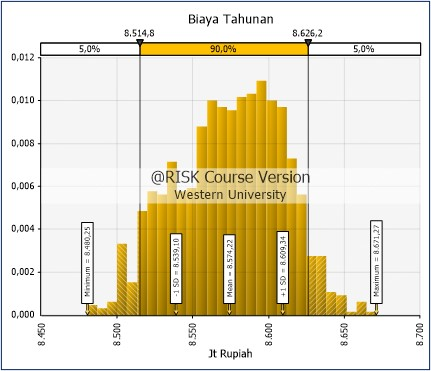
\includegraphics[width=\textwidth]{grafik/biaya-tahunan-baru.jpg}
        \caption{Tanpa Tangki}
    \end{subfigure}
    \hspace{0.04\textwidth}  % This adds horizontal spacing between images
    \begin{subfigure}{0.4\textwidth}
        \centering
        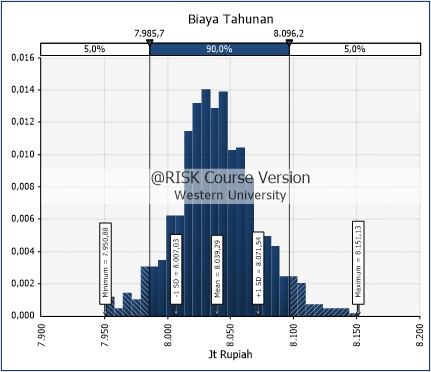
\includegraphics[width=\textwidth]{grafik/biaya-tahunan-baru-tangki.jpg}
        \caption{Dengan Tangki}    
    \end{subfigure}
    \caption{Hasil Simulasi Biaya}
    \label{fig:annual-cost-dist}
\end{figure}

\subsection{Analisis Kemungkinan Jumlah Perjalanan Tahunan}
\label{subsec:annual-freq-dist}

Frekuensi perjalanan setiap tahun dipengaruhi oleh angka konsumsi BBM harian dari setiap jenisnya. Model yang dibuat menentukan angka frekuensi berdasarkan ketika salah satu setiap jenis BBM habis dikonsumsi di salah satu titik maka harus diadakan pemasokan. Frekuensi tahunan akan mempengaruhi biaya tahunan dari sisi tambahan biaya perjalan yang muncul ketika kapal mengadakan pemasokan.

\begin{figure}[!ht]
    \centering
    \begin{subfigure}{0.4\textwidth}
        \centering
        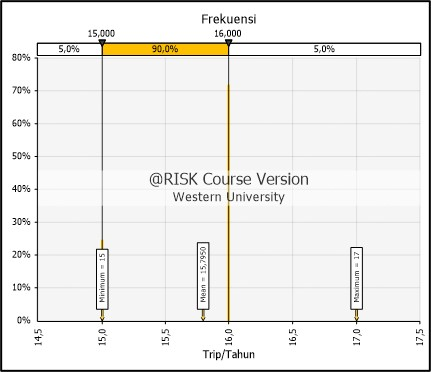
\includegraphics[width=\textwidth]{grafik/frekuensi-baru.jpg}
        \caption{Tanpa Tangki}
    \end{subfigure}
    \hspace{0.04\textwidth}  % This adds horizontal spacing between images
    \begin{subfigure}{0.4\textwidth}
        \centering
        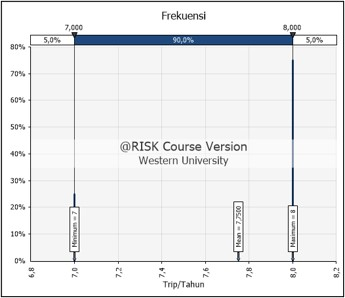
\includegraphics[width=\textwidth]{grafik/frekuensi-baru-tangki.jpg}
        \caption{Dengan Tangki}    
    \end{subfigure}
    \caption{Hasil Simulasi Frekuensi}
    \label{fig:annual-freq-dist}
\end{figure}

Gambar \ref{fig:annual-freq-dist} memperlihatkan bahwa kemungkinan terbesar perjalanan setiap tahunnya ada 9 perjalanan diikuti oleh 8 dan 10 untuk batas nilai kepercayaan 90\%. Meskipun begitu masih terlihat kemungkinan walauun sangat kecil di angka 19 perjalanan dalam satu tahun, hal ini mungkin terjadi ketika terjadi peningkatan konsumsi secara tiba-tiba pada setiap titik secara bergantian. Namun, seperti yang dimodelkan peluangnya sangat kecil.


\subsection{Analisis Kemungkinan Kelangkaan BBM}
\label{subsec:stock-out-over-capacity}

Gambar \ref{fig:potensi-bbm-overcap} menggambarkan seperti apa kemungkinan terjadinya BBM tidak mampu diangkut oleh kapal. Hal ini mungkin terjadi ketika angka konsumsi tinggi sehingga volume tangki yang tersedia di kapal tidak mencukupi. BBM jenis solar terlihat tidak mungkin terjadi muatan tidak terbawa, jika kita lihat pada kapasitas tangki yang tersedia dan dsitribusi konsumsi harian solar maka grafik tersebut menjadi masuk akal. Jenis BBM yang mempunyai kemungkinan besar untuk tidak terangkut adalah minyak tanah, dikonfirmasi oleh gambar \ref{fig:load-factor-bbm-pertrip} yang memperlihatkan kemungkinan \emph{load factor} minyak tanah yang lebih dari 100\%.

\begin{figure}[htbp!]
    \centering
    \begin{minipage}{\textwidth}
        \centering
        \begin{subfigure}[b]{0.9\textwidth}
            \centering
            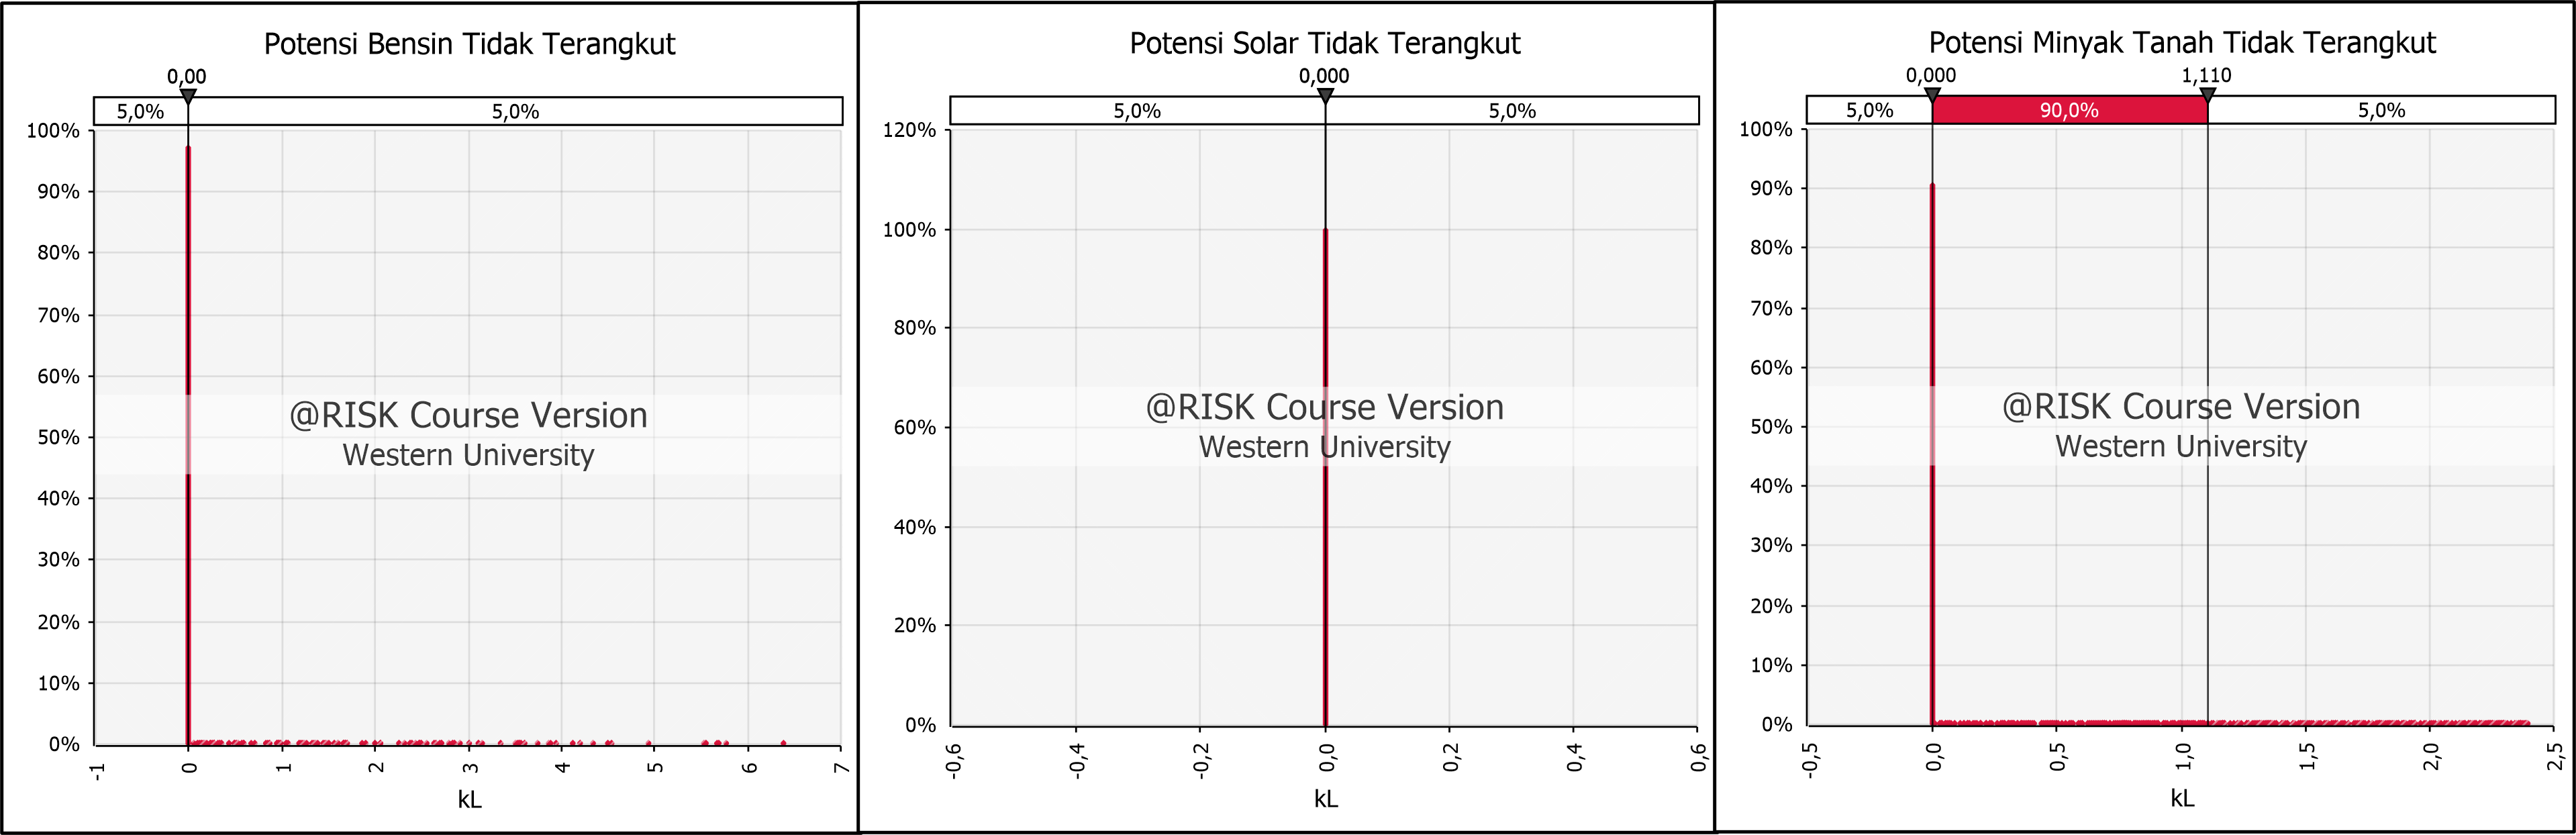
\includegraphics[width=\textwidth]{gambar/potensi-bbm-overcap.png}
            \caption{Distribusi Kumulatif Volume BBM tidak Terangkut oleh Kapal}
            \label{fig:potensi-bbm-overcap}
        \end{subfigure}
    \end{minipage}
    
    \vspace{1em} % Adjust the space between the subfigures as needed
    
    \begin{minipage}{\textwidth}
        \centering
        \begin{subfigure}[b]{0.9\textwidth}
            \centering
            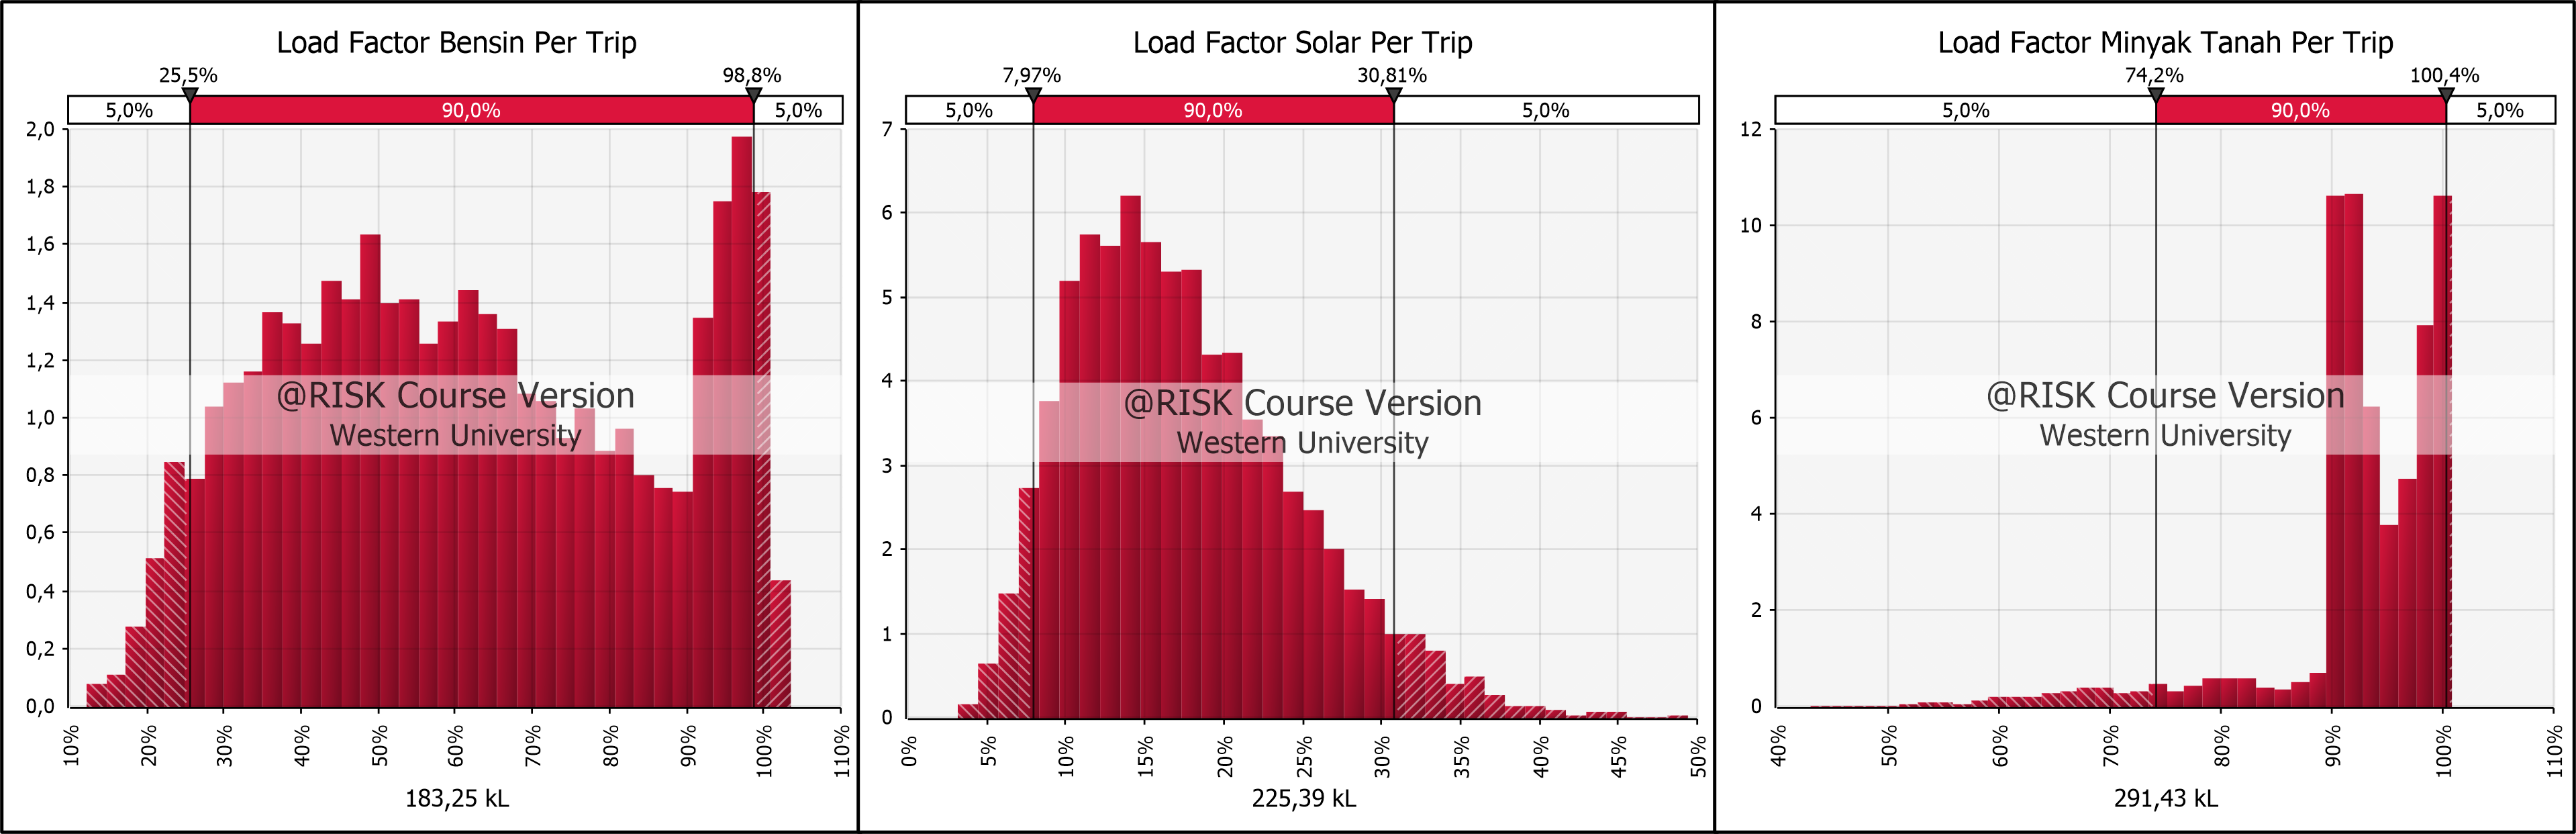
\includegraphics[width=\textwidth]{gambar/loadfactor-bbm-pertrip.png}
            \caption{\emph{Load Factor} setiap Jenis BBM}
            \label{fig:load-factor-bbm-pertrip}
        \end{subfigure}
    \end{minipage}
    \caption{Grafik Distribusi Kumulatif \emph{Load Factor} dan \emph{Over Capacity} BBM}
    \label{fig:grafik-analisis-overcap-BBM}
\end{figure}

Namun yang menjadi catatan menarik adalah jika dilihat dari sisi keseluruhan volume yang tersedia maka nilai \emph{load factor} kapal terbilang rendah (gambar \ref{fig:load-factor-kapal-overall}. Hal ini berbanding lurus dengan distribusi konsumsi harian solar dan bensin (gambar \ref{fig:all-bbm-graphs}) yang cenderung condong ke kiri ke nilai yang lebih kecil sedangkan minyak tanah cenderung normal atau berada di titik paling mungkin.

\begin{figure}[htbp!]
    \centering
    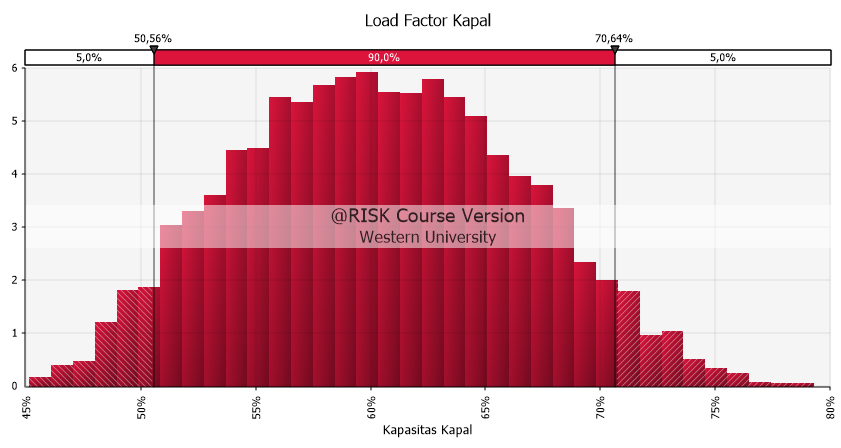
\includegraphics[width=0.8\textwidth]{gambar/loadfactor-ship-overall.png}
    \caption{Grafik Distribusi Kumulatif \emph{Load Factor} Kapal Keseluruhan}
    \label{fig:load-factor-kapal-overall}
\end{figure}


\subsection{Perhitungan Kebutuhan Tangki Tambahan}
\label{subsec:hitungan-tangki}

Konsekuensi dari sistem yang diusulkan yakni mengurangi frekuensi kunjungan kapal adalah adanya persediaan BBM yang cukup antar kedatangan kapal. Formulasi yang digunakan untuk menghitung kebutuhan tangki adalah penyimpanan tersedia saat ini dikurangi perkalian dari jeda hari antar pemasokan dengan konsumsi harian kemudian dibulatkan keatas menyesuaikan ukuran tangki yang tersedia. Rekapitulasi kebutuhan tangki tambahan dapat dilihat pada tabel \ref{rekapitulasi-tambahan-tangki}.

\begin{table}[!htbp]
    \centering
    \caption{Rekapitulasi Tambahan Tangki yang Dibutuhkan}
    \begin{tabular}{|l|c|c|c|}
    \hline
        \textbf{Lokasi} & \textbf{Minyak Tanah [kL]} & \textbf{Solar [kL]} & \textbf{Bensin [kL]} \\ \hline
        Lakor & 50 & 0 & 0 \\ \hline
        Letti & 50 & 0 & 0 \\ \hline
        Romang & 50 & 0 & 0 \\ \hline
        Tiakur & 170 & 50 & 0 \\ \hline
        Tepa & 70 & 10 & 0 \\ \hline
    \end{tabular}
    \label{rekapitulasi-tambahan-tangki}
\end{table}

